% Author: Izaak Neutelings (October 2017)
% https://tex.stackexchange.com/questions/44505/export-tikz-figures-to-pdf
% add "--shell-escape" to latex command in Preferences > Engine
\documentclass[border=2pt,varwidth,10pt]{standalone}
\usepackage{amsmath,amssymb}
\usepackage{bm} % math bold
\usepackage[outline]{contour} % glow around text
\contourlength{1.2pt}

\usepackage{tikz}
\usetikzlibrary{external}
\usetikzlibrary{patterns}
%\tikzset{external/mode=graphics if exists} % prevents mysterious errors
\tikzexternalize %[force remake] % activate external
\usepackage{pgfplots} % for the axis environment
\tikzset{>=latex}
\usetikzlibrary{calc}
\usetikzlibrary{angles,quotes} % for pic

\begin{document}



% EXERCISE 1 setup without axes
\def\setup{
  \def\N{20}
  \def\depth{0.25}
  \def\h{6} % height balcony
  \def\w{2} % width ground
  \def\wb{\depth*3} % width balcony
  \def\xland{(\w-\wb*0.8)} % x component of landing position
  \def\xmin{-\depth*3}
  \def\xmax{\w+\depth*3.0}
  \def\ymin{-\depth*3}
  \def\ymax{\h*1.2}
  \def\tmin{0}
  \def\tmax{\xland}
  \def\a{-4.0} % parabola amplitude
  \def\c{(\xland-\h/\xland/\a)} % parabola parameter

  % ground, wall, balcony
  \draw[draw=none,pattern color=black!70!white,pattern=north east lines]
    (0,0) -- (0,-\depth) -- (\w+\depth,-\depth) 
      -- (\w+\depth,\h*1.1) -- (\w,\h*1.1) -- (\w,0) -- cycle;
  \draw[thick,black!70!white]
    (0,0) -- (\w,0) -- (\w,\h*1.1);
  \draw[thick,black!70!white,pattern color=black!70!white,pattern=north east lines]
    (\w-\wb,\h-\depth*4) rectangle (\w,\h);
  
  % parabola
  \draw[very thick,black!40!blue,variable=\t,domain=0:\tmax,samples=\N,smooth]
    plot (\t,{\a*\t*(\t-\c)});
}



% EXERCISE 1 setup with axes
\tikzsetnextfilename{ex1-setup}
\begin{tikzpicture}[scale=0.8]
  \setup % axes
  \draw[thick,->] (\xmin,0) -- (\xmax,0) node[anchor=north]       {$x\,[\text{m}]$};
  \draw[thick,->] (0,\ymin) -- (0,\ymax) node[anchor=north east]  {$y\,[\text{m}]$};
  \fill (0,0) circle[radius=2.5pt] node[below left=-1pt] {0};
  \draw[thick]    (+\depth/2,\h) -- (-\depth/2,\h) node[left] {$h$};
\end{tikzpicture}



% EXERCISE 1 setup with axes 2
\tikzsetnextfilename{ex1-setup2}
\begin{tikzpicture}[scale=0.8]
  \setup % axes
  \draw[thick,->] (\xmin,\h) -- (\xmax,\h) node[left=6pt,anchor=north west] {$x\,[\text{m}]$};
  \draw[thick,->] (0,\ymin)  -- (0,\ymax)  node[anchor=north east] {$y\,[\text{m}]$};
  \fill (0,\h) circle[radius=2.5pt] node[below left=-1pt] {0};
  \draw[thick]    (+\depth/2,0) -- (-\depth/2,0) node[left] {$-h$};
\end{tikzpicture}



% EXERCISE 1 setup with axes 3
\tikzsetnextfilename{ex1-setup3}
\begin{tikzpicture}[scale=0.8]
  \setup % axes
  \draw[thick,->] (\xmin,\h) -- (\xmax,\h) node[left=6pt,anchor=north west] {$x\,[\text{m}]$};
  \draw[thick,->] (0,\ymax) -- (0,\ymin) node[below=4pt,anchor=south east] {$y\,[\text{m}]$};
  \fill (0,\h) circle[radius=2.5pt] node[below left=-1pt] {0};
  \draw[thick]    (+\depth/2,0) -- (-\depth/2,0) node[above=2pt,left] {$h$};
\end{tikzpicture}



% EXERCISE 2
\tikzsetnextfilename{ex2-setup}
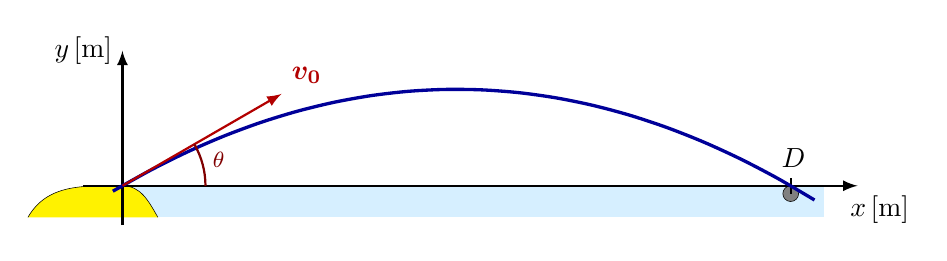
\begin{tikzpicture}[scale=0.5]
  \def\N{20}
  \def\vi{14}
  \def\g{10}
  \def\thetaI{30}
  \def\D{\vi^2*sin(2*\thetaI)/\g} %15
  \def\ymax{\vi^2*sin(\thetaI)^2/(2*\g)*1.4}
  \def\xmax{\D*1.1}
  \def\xmin{-1}
  \def\ymin{-1}
  \def\tmin{-0.02}
  \def\tmax{(2*\vi*sin(\thetaI)/\g)+0.05}
  
  % water, beach & rock
  \fill[blue!40!cyan!40!white!40]
    (0,0) rectangle ({(\xmax+\D)/2},\ymin*0.8);
  \draw[very thin,fill=yellow] %north east lines, crosshatch dots
    (\xmin*2.4,\ymin*0.8) to[out=60,in=180] (0,0) to[out=0,in=120] (-\xmin*0.9,\ymin*0.8);
  \draw[very thin,fill=black!50!white] %north east lines, crosshatch dots
    ({\D},-0.2) circle (0.2);
  
  % axes
  \draw[thick,->] (\xmin,0) -- ({\xmax},0) node[right=8pt,anchor=north] {$x\,[\text{m}]$};
  \draw[thick,->] (0,\ymin) -- (0,{\ymax}) node[anchor=east] {$y\,[\text{m}]$};
  \draw[thick] ({\D},-0.2) -- ({\D},0.2) node[right=1pt,above] {$D$}; 
  
  % parabola
  \draw[very thick,black!40!blue,variable=\t,domain=\tmin:\tmax,samples=\N,smooth]
    plot ({\vi*cos(\thetaI)*\t},{\vi*sin(\thetaI)*\t-\g*\t^2/2});
  
  % vectors
  \coordinate (O)   at (0,0);
  \coordinate (X)   at (1,0);
  \coordinate (V)   at ({\vi*cos(\thetaI)/3},{\vi*sin(\thetaI)/3});
  \coordinate (Vx)  at ({\vi*cos(\thetaI)/3},-0.1);
  \coordinate (Vy)  at (-0.1,{\vi*sin(\thetaI)/3});
%  \draw[dashed,black!10!red]
%    (V) -- (Vx)
%    node[below=-2pt] {\contour{white}{$v_0\cos\theta$}};
%  \draw[dashed,black!10!red]
%    (V) -- (Vy)
%    node[left] {$v_0\sin\theta$};
  \draw[->,black!30!red,thick]
    (O) -- (V)
    node[above right] {\contour{white}{$\bm{v_0}$}}; %=(v_0\cos\theta,v_0\sin\theta)
  
  % angles
  \pic[draw,thick,black!50!red,"\footnotesize$\theta$",angle radius=30,angle eccentricity=1.2]
    {angle = X--O--V};
  
\end{tikzpicture}



\tikzsetnextfilename{ex2-two_trajectories}
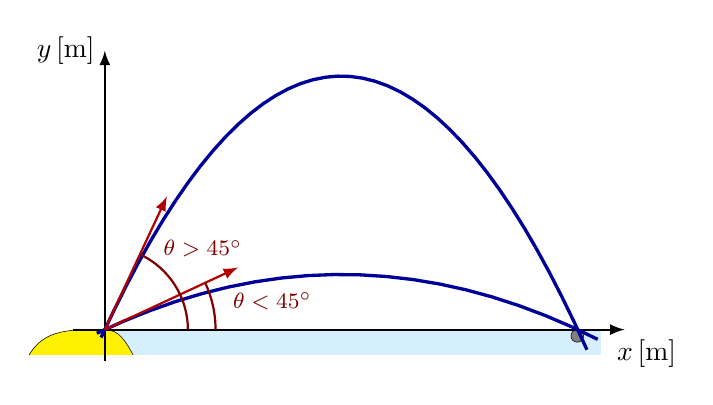
\begin{tikzpicture}[scale=0.4]
  \def\N{20}
  \def\vi{14}
  \def\D{15}
  \def\g{10}
  \def\thetaI{65}
  \def\thetaII{25}
  \def\ymax{{\vi^2*sin(\thetaI)^2/(2*\g)*1.1}}
  \def\xmax{\D*1.1}
  \def\xmin{-1}
  \def\ymin{-1}
  \def\tmin{-0.02}
  \def\tmaxI{(2*\vi*sin(\thetaI)/\g)+0.05}
  \def\tmaxII{(2*\vi*sin(\thetaII)/\g)+0.05}

  % water, beach & rock
  \fill[blue!40!cyan!40!white!40]
    (0,0) rectangle ({(\xmax+\D)/2},\ymin*0.8);
  \draw[very thin,fill=yellow] %north east lines, crosshatch dots
    (\xmin*2.4,\ymin*0.8) to[out=60,in=180] (0,0) to[out=0,in=120] (-\xmin*0.9,\ymin*0.8);
  \draw[very thin,fill=black!50!white] %north east lines, crosshatch dots
    (\D,-0.2) circle (0.2);
  
  % axes
  \draw[thick,->] (\xmin,0) -- (\xmax,0) node[right=8pt,anchor=north] {$x\,[\text{m}]$};
  \draw[thick,->] (0,\ymin) -- (0,\ymax) node[anchor=east] {$y\,[\text{m}]$};
  
  % parabola
  \draw[very thick,black!40!blue,variable=\t,domain=\tmin:\tmaxI,samples=\N*2]
    plot ({\vi*cos(\thetaI)*\t},{\vi*sin(\thetaI)*\t-\g*\t^2/2});
  \draw[very thick,black!40!blue,variable=\t,domain=\tmin:\tmaxII,samples=\N]
    plot ({\vi*cos(\thetaII)*\t},{\vi*sin(\thetaII)*\t-\g*\t^2/2});

  % vectors
  \coordinate (O)   at (0,0);
  \coordinate (X)   at (1,0);
  \coordinate (V)   at ({\vi*cos(\thetaII)/3},{\vi*sin(\thetaII)/3});
  \coordinate (V')  at ({\vi*cos(\thetaI)/3}, {\vi*sin(\thetaI)/3});
  \coordinate (Vx)  at ({\vi*cos(\thetaII)/3},0);
  \coordinate (Vx') at ({\vi*cos(\thetaI)/3}, 0);
  \draw[->,black!30!red,thick] (O) -- (V);
  \draw[->,black!30!red,thick] (O) -- (V');
  
  % projections
  %\draw[dashed,black!20!red] (Vx)  -- (V);
  %\draw[dashed,black!20!red] (Vx') -- (V');
  
  % angles
  \pic[draw,thick,black!50!red,angle radius=40,angle eccentricity=1.2]
    {angle = X--O--V};
  \pic[black!50!red,"\footnotesize$\theta<45^\circ$" right=-4pt,
       angle radius=40,angle eccentricity=1.2]
    {angle = X--O--V};
  \pic[draw,thick,black!50!red,angle radius=30,angle eccentricity=1.2]
    {angle = X--O--V'};
  \pic[black!50!red,"\footnotesize$\theta>45^\circ$" above,
       angle radius=35,angle eccentricity=1.2]
    {angle = X--O--V'};
\end{tikzpicture}



% NUMERICAL SOLUTIONS
\tikzsetnextfilename{ex2-numerical_solution}
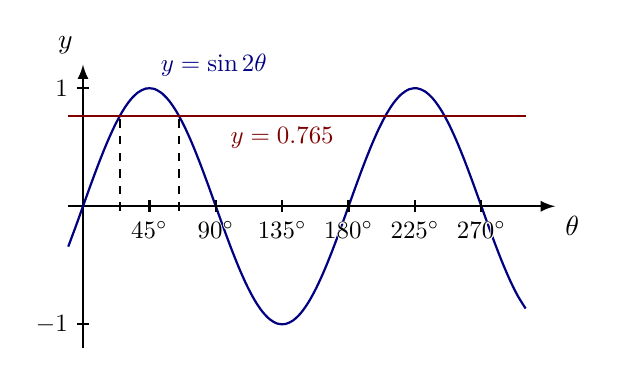
\begin{tikzpicture}[scale=1.5,xscale=1/80]
  
  \def\N{60}
  \def\xmin{-10}  \def\xmax{320}
  \def\ymin{-1.2} \def\ymax{1.2}
  \def\tmin{-10}  \def\tmax{300}
  \def\blue{black!50!blue}, \def\red{black!50!red}
  \def\value{0.765}
  \def\Dtheta{20}
  
  % axes
  \draw[->,thick]
    (\xmin,0) -- (\xmax,0)
    node[anchor=north west] {$\theta$};
  \draw[->,thick]
    (0,\ymin) -- (0,\ymax)
    node[anchor=south east] {$y$};
  
  % plots
  \draw[thick,\blue,variable=\t,domain=\tmin:\tmax,samples=\N,smooth]
    plot (\t,{sin(2*\t)});
  \draw[thick,\red,variable=\t,domain=\tmin:\tmax,samples=\N,smooth]
    plot (\t,\value);
  
  % function labels
  \node[\blue,above right=1pt,scale=0.9] at (45,1) {$y=\sin2\theta$};
  \node[\red, below=1pt,scale=0.9] at (135,\value) {$y=\value$};
  
  % numerical solutions
  \draw[dashed,thick] (45-\Dtheta,-\value*0.05) -- (45-\Dtheta,\value*1.05);
  \draw[dashed,thick] (45+\Dtheta,-\value*0.05) -- (45+\Dtheta,\value*1.05);
  
  % ticks
  \foreach \x in {45,90,135,180,225,270}{
    \draw[thick]
      (\x,0.05) -- (\x,-0.05) node[below,scale=0.9] {\contour{white}{$\x^\circ$}};}
  \foreach \y in {1,-1}{
    \draw[thick]
      (4,\y) -- (-4,\y) node[left,scale=0.9] {$\y$};}
   
\end{tikzpicture}



\end{document}